\documentclass[12pt a4paper]{paper}
\usepackage{float}
\usepackage{graphicx}
\usepackage{fancyhdr}
\usepackage[utf8]{inputenc}
\graphicspath{{./images/}}

% Cover Text Elements
\title{\center{Teoria dos Grafos}}
\author{João Vitor Rezende Moura}
\date{2023-10-29}
% Page Style Configurations

\pagestyle{fancy}
\fancyhead{}
\fancyfoot{}
\fancyhead[L]{UNIT - Universidade Tiradentes}
\fancyhead[R]{2023-10-29}
\fancyfoot[C]{\thepage}

% --- Document ---
\begin{document}

\maketitle
\begin{abstract}
Algoritmos e Grafos são de suma importância dentro do campo computacional devido à importância do seu uso, tanto no campo teórico, como no prático. Devido o seu foco computacional, a eficiência de tempo e espaço dos processos são fundamentais devido à sua aplicação posterior dentro da computação.
É de importância, o estudo de tópicos tanto básicos, como técnicas elementares, busca em grafo, otimização combinatória, como tópicos mais avançados, como estudo de complexidade, e estudo do problema de fluxo máximo.
Com isso, a resolução de exercícios também é de suma importância, e será apresentado.
\end{abstract}

\section{História dos Grafos}
Temos como a área de estudo da computação que é voltada para os grafos, o objetivo de encontrar algoritmos eficientes para resolver problemas relacionados a grafos. Sendo assim, existem diferenças entre esa área, e a teoria dos grafos, algumas dessas diferenças são:

\begin{itemize}
  \item Há problemas não algorítmicos em grafos que sua eficiência é sem sentido.
  \item A preocupação pela eficiência, na área de algoritmos, se traduz na formulação de problemas em grafos que talvez se encontrem fora do interesse da teoria.
\end{itemize}
Temos como principal e precursor problema da teoria dos grafos, o \textit{problema da ponte de Konigsberg}, que hoje em dia é conhecida como Kaliningrado, na então Prússia. Nela existiam duas ilhas que entre elas, haviam um total de 7 pontes que conectavam elas, às duas margens que as rodeavam, o problema se resume, em a partir de qualquer um dos pontos, fazer um percurso que retorne ao mesmo, passando por todas as pontes, apenas uma vez. 
Observou-se que esse problema não havia solução, pois as pontes possuiam uma disposição específica que tornava impossível resolver esse problema, e essa disposição foi a seguinte:

\begin{figure}[H]
\centering
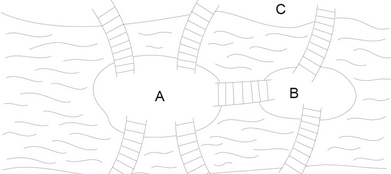
\includegraphics[scale=0.8]{Konigsberg}
\caption{Problema da ponte de Konigsberg}
\end{figure}

Pelo fato das ilhas C e B possuirem uma quantidade ímpar de pontes conectadas a elas, esse problema se torna impossível de ser solucionado, devido à natureza do deslocamento por essas duas pontes.
Com esse problema, outros foram aparecendo, e com isso desenvolvimentos importantes foram sendo criados, como por exemplo o \textit{problema das quatro cores de Francis Guthrie} e o \textit{problema do ciclo Hamiltoniano}.

\subsection{Problema das quatro cores}
O problema das quatro cores consiste em colorir os países de um mapa arbitrário plano, em que cada país tem uma cor e seus fronteiriços possuam necessariamente cores diferentes dele, e o problema consiste em colorir eles de forma que não utilize mais que 4 cores, esse problema foi resolvido em 1977 por Appel e Hakeo problema das quatro cores consiste em colorir os países de um mapa arbitrário plano, em que cada país tem uma cor e seus fronteiriços possuam necessariamente cores diferentes dele, e o problema consiste em colorir eles de forma que não utilize mais que 4 cores, esse problema foi resolvido em 1977 por Appel e Haken

\subsection{Problema do ciclo hamiltoniano}
Possuindo uma quantidade \textit{n} de cidades. Cada par de cidades pode ser adjacente, ou não. Determine um trajeto que passe por cada cidade apenas uma vez e que retorne ao ponto de partida, tal que cada par de cidades consecutivas no trajeto seja sempre uma adjacente, partindo de uma cidade qualquer.
Esse problema ainda não possui solução satisfatória, pelo fato de ser necessário analisar todas as poermutações existentes.

\section{Introdução à Teoria dos Grafos}
\subsection{Conceitos Iniciais}
Um grafo \textit{G (V, E)}, pode ser definido como m conjunto finito não vazio de vértices \textit{V}, e de arestas \textit{E}, de pares não ordenados dos elementos distintos de \textit{V}. Temos como uma características singulares do grafo, as seguintes:
\begin{itemize}
  
  \item A nomeclatura de \textit{grafo trivial} quando temos \textbar \textit{V} \textbar = 1.
  \item Quando necessário, utiliza-se o termo \textit{Grafo não direcionado} para designar um grafo.
  \item Temos para cada aresta $ e \in E \; \forall \; e = (v, w) $ sendo eles as extremidades dos vértices que formam aquela aresta
  \item A aresta é dita \textit{incidente} a ambos v,w. Dias arestas que possuem um extremo comum são chamadas de adjacentes.

\end{itemize}

Um grafo pode ser visualizado através de uma representação geométrica, na qual seus vértices correspondem a pontos distintos do plano em posições arbitrárias, enquanto a cada aresta (v, w) é associada uma linha arbitrária de exposição, é usuap confundir-se um grafo com a sua representação geométrica.\par
Algumas vezes é útil relaxar a definição de grafos, de modo a permitir uma aresto do tipo $e = (v, v)$, isto é, formada por um par de vértices idênticos. Uma aresta desta natureza é chamada de laço. Uma outra extensão possível consiste em substituir, na definição de grafo, o conjunto de arestas \textit{E} por um multiconjunto. O efeito desta alteração é, naturalmente, permitir a existência de mais de uma aresta entre o mesmo par de vértices, as quais são então, denominadas arestas paralelas.\par

\subsubsection{Definições específicas quanto à forma de construção e forma de visualizar e relacionar os vértices por meio das arestas} % (fold)
\label{sec:Definições específicas quanto à forma de construção e forma de visualizar e relacionar os vértices por meio das arestas}
Podemos dizer que o \textit{grau de um vértice} é a quantidade de vértices adjacentes conectados a ele. Com isso, podemos dizer que um grafo é \textbf{\textit{regular}} quando todos os seus vértices possuírem o mesmo grau de conexões.\par
Uma sequência de vértices pode receber diversas denominações a depender da forma como elas se conectam e se comportam. Temos que a sequẽncia de vértices é denominada de \textbf{\textit{caminho ou passeio}}. Entretanto, quando temos um caminho o qual o número \textit{k} de vértices é formado por \textit{k - 1} arestas, temos que esse valor é o \textit{comprimento} do caminho. \par
A partir do caminho que é dado por uma sequência de vértices de um grafo, podemos definir se, caso todos os vértices do caminho forem distintos, a sequência recebe a denominação de \textit{\textbf{simples ou elementar}}, e se todas as arestas forem distintas, podemos denominar o caminho como um \textbf{\textit{trajeto}}.\par
Um caminho pode ser considerado um ciclo, se ele, possuir no mínimo três vértices, e volte ao primeiro ao fim do seu passeio. Caso o grafo não possua o mesmo, ele é considerado \textbf{\textit{acíclico}}. Dentro dessa classificação possuem duas subclassificações, que são os ciclos \textbf{hamiltoniano} ou \textbf{euleriano}, e oque difere eles é que no ciclo os vértices são acessados uma única vez, e as arestas são acessadas uma única vez, respectivamente.\par % (fold)
Uma denominação importante para o estudos do grafo, e para algumas finalidades de pesquisa que ele pode ter, é em relação à sua conexicidade

% paragraph  (end) 
% subsubsection Definições específicas quanto à forma de construção e forma de visualizar e relacionar os vértices por meio das arestas (end)


\end{document}
